\documentclass[12pt,fleqn]{article}
\setlength{\parindent}{0pt}
\usepackage{graphicx}
\usepackage{cancel}
\usepackage{listings}
\usepackage[latin5]{inputenc}
\usepackage{color}
\setlength{\parskip}{8pt}
\setlength{\parsep}{0pt}
\setlength{\headsep}{0pt}
\setlength{\topskip}{0pt}
\setlength{\topmargin}{0pt}
\setlength{\topsep}{0pt}
\setlength{\partopsep}{0pt}
\setlength{\mathindent}{0cm}

\begin{document}
Cok Degiskenli Calculus - Ders 20

Cizgi entegrallerini is hesabinda gormustuk. $\vec{F}$ tarafindan $C$
egrisi uzerinde yapilan isi

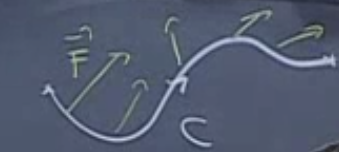
\includegraphics[height=2cm]{20_1.png}

\[ \int_C \vec{F} \cdot d\vec{r} =  \int_C \vec{F} \cdot \vec{T} ds \]

olarak gormustuk. Esitligin sagi birim teget vektoru kullanarak ayni hesabi
gosteriyor, $ds$ ise egri uzunlugu $s$'ten ortaya cikiyor. Diger bir form

\[ = \int_C M dx + N dy \]

ki $\vec{F} = <M,N>$ olmak uzere. 

Ornek 

Soyle bir vektor alani veriyorum

\[ \vec{F} = <y,x> \]

Bu alanin neye benzedigi cok bariz degil, ama bu alanin bir bilgisayar
cizimi altta

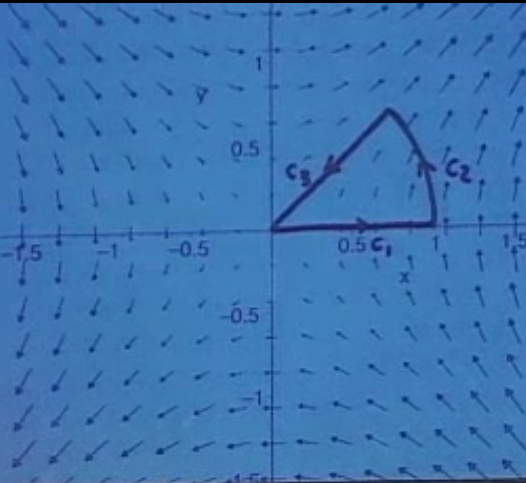
\includegraphics[height=5cm]{20_2.png}







\end{document}
